%
% Copyright (c) 2013-2023 Aleksey Fedoseev <aleksey@fedoseev.net>
% Copyright (c) 2015-2016 Alexander Shaenko <ark4110@gmail.com>
% Copyright (c) 2016-2023 Ilya Tagunov <tagunil@gmail.com>
% 
% Permission is granted to copy, distribute and/or modify this document
% under the terms of the GNU Free Documentation License, Version 1.3
% or any later version published by the Free Software Foundation;
% with no Invariant Sections, no Front-Cover Texts, and no Back-Cover Texts.
% A copy of the license is located here: http://www.gnu.org/copyleft/fdl.html.
%

\documentclass[12pt,a4paper]{article}
\usepackage[T2A]{fontenc}
\usepackage{ucs}
\usepackage[utf8]{inputenc}
\usepackage[english,russian]{babel}
\usepackage{indentfirst}
\usepackage{amsmath}
\usepackage{amssymb}
\usepackage{gensymb}
\usepackage{graphicx}
\usepackage{hyperref}
\usepackage{array}
\usepackage{titlesec}
\usepackage{subcaption}
\usepackage{wasysym}
\usepackage{longtable}
\usepackage{multirow}

\pagestyle{plain}
\parindent=1.25cm
\textheight=24cm
\textwidth=16cm
\topmargin=-1cm
\frenchspacing
\renewcommand{\theequation}{\thesection.\arabic{equation}}
\newcommand{\sectionbreak}{\clearpage}

\begin{document}

\title{%
  \textbf{Инженерный симулятор ОРБИТА 2.0} \\
    Руководство для преподавателя}

\author{
  Алексей Федосеев\\
  \texttt{aleksey@fedoseev.net}
  \and
  Александр Шаенко\\
  \texttt{ark4110@gmail.com}
  \and
  Илья Тагунов\\
  \texttt{tagunil@gmail.com}
}

\date{Версия 1.1, \today}

\maketitle

Этот текст распространяется под лицензией GNU Free Documentation License (FDL) версии
1.3. Подробную информацию об этой лицензии Вы можете на сайте GNU
\footnote{\url{http://www.gnu.org/copyleft/fdl.html}}.

Исходный текст находится в репозитории проекта на GitHub
\footnote{\url{https://github.com/dralex/orbita-simulator}}.

\tableofcontents

\clearpage
\section{Введение}

Симулятор «Орбита» позволяет спроектировать космический аппарат (КА), который должен
решить поставленную прикладную задачу на околоземной орбите. КА конструируется в виде
набора общих параметров и выбора подсистем, которые должны соответствовать общим
требованиям и решаемой задаче.

Симулятор позволяет рассчитать параметры КА в течение всего полёта и отображает переданную
на Землю телеметрию и результат полёта.

\subsection{Описание миссий}

Симулятор позволяет последовательно проходить следующие миссии:

\begin{description}
  \item[Тренировочная-1: Смотрим на Землю] КА стартует на орбите заданной
    высоты. Необходимо погасить начальное вращение аппарата и совершить полный оборот
    Земли с ориентацией аппарата в надир (нормально по отношению к поверхности). В этой
    тренировочной миссии аппарат будет полностью сконструирован, нужно будет только
    произвести расчёты и вставить в программу полёта нужные константы.
  \item[Тренировочная-2: Связь с Землёй] КА стартует на орбите заданной
    высоты. Необходимо запрограммировать аппарат для отправки сообщения на Землю через
    подсистему высокопроизводительной связи. В этой тренировочной миссии аппарат будет
    полностью сконструирован, нужно будет только написать его программу полёта.
  \item[Тренировочная-3: Орбитальный манёвр] КА стартует на орбите заданной
    высоты. Необходимо запрограммировать аппарат для перехода на более высокую орбиту. В
    этой тренировочной миссии аппарат будет полностью сконструирован, нужно будет только
    рассчитать необходимую массу топлива и написать программу полёта.
  \item[Дистанционное зондирование Земли] КА стартует на орбите заданной высоты. Вам
    необходимо сделать из космоса снимок объекта расположенного на Земле. Данные снимка
    нужно передать в наземный измерительный пункт (НИП) по высокопроизводительному каналу
    связи. Количество полученных победных очков зависит от разрешения снимка и
    нормальности ориентации аппарата по отношению к поверхности в момент съёмки.
  \item[SMS везде] КА стартует на орбите заданной высоты. Команде выдаётся набор
    сообщений, которые должны быть доставлены между НИП-ами. Необходимо последовательно
    переориентировать аппарат на НИП-ы, чтобы принять сигнал от одних станций и передать
    его на другие. Количество полученных победных очков зависит от числа переданных на
    Землю сообщений.
  \item[Инспекция спутника] КА стартует на орбите заданной высоты. Известна другая орбита,
    по которой движется спутник-цель. Необходимо приблизиться к цели, чтобы
    сфотографировать его и передать результаты съёмки на Землю. Количество полученных
    победных очков зависит от разрешения снимка.
  \item[Белковый кристалл в невесомости] КА стартует на орбите заданной высоты. Ваша
    задача – вырастить в невесомости белковый кристалл и доставить его на Землю. Для этого
    Вам нужно вывести спутник на заданную орбиту, сделать один оборот вокруг планеты с
    выключенной аппаратурой (включёнными могут быть только бортовая вычислительная
    система, подсистема электропитания и сам контейнер с кристаллом), сохраняя температуру
    КА в требуемом диапазоне, а затем посадить аппарат в определённую точке земной
    поверхности. Количество полученных победных очков зависит от точности посадки.
\end{description}

В данном руководстве мы опишем принципы конструирования КА, а также все используемые в
симуляторе математические модели. Вы также сможете познакомиться с подробным описанием и
условиями миссий в разделе \ref{Sec:Missions}.

\section{Конструирование аппарата}

КА представляется в виде систем-блоков, описываемых набором параметров и объединённых
различного рода связями. Для моделирования доступны следующие десять блоков (подсистем),
семь из которых являются обязательными для любого КА (см. рисунок \ref{Pic:subsystems}).

\begin{figure}[tbh]
  \begin{center}
    \includegraphics[width=12cm]{images/subsystems-ru.eps}
    \caption{Схема подсистем КА}
    \label{Pic:subsystems}
  \end{center}
\end{figure}

Каждая из подсистем характеризуется следующим набором параметров:

\begin{itemize}
\item масса (кг);
\item объем (л);
\item допустимый температурный режим: мин./макс. (°С);
\item энергопотребление (Вт);
\item тепловыделение (Вт);
\item текущее состояние (вкл., выкл., неисправно).
\end{itemize}

Рассмотрим подробнее назначение каждой из подсистем и их специальные параметры
(\textbf{*}~--- обязательная подсистема):

\begin{description}
\item[Конструктив (корпус) аппарата (*)] Корпус составляет внешний контур КА, а также
  используется для монтажа всех систем КА. К специальным параметрам конструктива
  относится:
  \begin{itemize}
    \item размер стороны куба, м.
  \end{itemize}
\item[Бортовая вычислительная система (*)] БВС содержит основную программу полёта и набор
  служебных параметров. К специальным параметрам БВС относится:
  \begin{itemize}
    \item оперативная память, МБ.
  \end{itemize}
\item [Система электропитания (*)] Система электропитания (СЭ) обеспечивает электрической энергией
  все системы КА. Как правило эта система состоит из аккумулятора и набора солнечных
  батарей, а также системы управления питанием. К специальным параметрам СЭ относятся:
  \begin{itemize}
  \item ёмкость аккумулятора, $\text{Вт} - \text{ч}$;
  \item КПД солнечных батарей, \%;
  \item коэффициент поглощения тепла солнечными батареями;
  \item коэффициент черноты солнечных батарей.
  \end{itemize}

\item [Система навигации (*)] Система навигации содержит специальный вычислитель и набор
  датчиков, позволяющих с высокой точностью определить положение аппарата относительно
  Земли. Не имеет специальных параметров.

\item [Система управления ориентацией и стабилизацией (*)] Система управления ориентации и
  стабилизацией (СУОС) обеспечивает ориентацию аппарата в заданном направлении. К
  специальным параметрам СУОС относится:
  \begin{itemize}
    \item максимальный момент, $\text{Н} \cdot \text{м}$.
  \end{itemize}

\item [Система обеспечения теплового режима (*)] Система обеспечения теплового
  режима (СОТР) служит для поддержания требуемого температурного режима аппарата. Как правило,
  эта система содержит датчики температуры, нагреватели и радиатор, который может излучать
  излишки тепла в космическое пространство. К специальным параметрам СОТР относятся:
  \begin{itemize}
  \item коэффициент поглощения тепла радиаторами;
  \item коэффициент черноты радиатора;
  \item мощность нагревателя, Вт.
  \end{itemize}

\item [Система телеметрии (*)] Система телеметрии предназначена для передачи на Землю
  служебных сообщений о состоянии аппарата и его систем. Как правило, эта система содержит
  независимый передатчик малой мощности. К специальным параметрам системы телеметрии
  относятся:
  \begin{itemize}
  \item усиление бортовой антенны;
  \item усиление наземной антенны;
  \item угол раскрыва антенны, °;
  \item мощность передатчика, Вт.;
  \item частота (МГц)
  \end{itemize}
  
\item [Система высокопроизводительной связи] Система высокопроизводительной связи
  позволяет передавать на Землю данные большого объёма за короткие периоды
  времени. Система высокопроизводительной связи имеет те же специальные параметры, что и
  система телеметрии (см. выше).

\item [Система изменения орбиты] Система изменения орбиты содержит двигательную установку
  и топливные баки.
  \begin{itemize}
    \item максимальный массовый расход топлива, кг/с;
    \item удельный импульс двигательной установки, м/с;
    \item объем топливных баков, л.
  \end{itemize}

\item [Полезная нагрузка (вариант 1~--- камера)] Камера позволяет производить цифровые
  снимки объектов на Земле и в космосе. К специальным параметрам камеры относятся:
  \begin{itemize}
  \item угол поля зрения, °;
  \item спектральный диапазон;
  \item поток данных, Мбит/с;
  \item объем памяти, МБ;
  \item матрица, пикс.
  \end{itemize}

\item [Полезная нагрузка (вариант 2~--- контейнер для кристалла)] Контейнер предназначен
  для выращивания белковых кристаллов и последующей их транспортировки на Землю. Контейнер
  содержит жаропрочные стенки, парашют и систему амортизации при посадке на
  Землю. Контейнер не имеет специальных параметров.

\end{description}

Полный список подсистем, доступных для конструирования, представлен в Приложении 1.

Корпус аппарата для простоты моделирования принимается за имеющий кубическую форму,
доступны корпуса разного размера. Таким образом, аппарат имеет шесть внешних поверхностей
(см. рисунок \ref{Pic:cube}).

\begin{figure}[tbh]
  \begin{center}
    \includegraphics[width=6cm]{images/cube.eps}
    \caption{Принципиальная пространственная модель КА}
    \label{Pic:cube}
  \end{center}
\end{figure}

Нумерация поверхностей с 1 по 4 идёт против часовой стрелки, поверхности 5 и 6 находятся в
плоскости X0Y, при этом поверхность 5 имеет большую координату по оси Z. С учетом того,
что в данной модели аппарат движется в плоскости X-Y, грани 5 и 6 всегда параллельны
плоскости движения аппарата.

Компоновка подсистема внутри аппарата в модели не рассматривается, однако некоторые
подсистемы имеют выводы на поверхности корпуса:

\begin{itemize}
\item антенна системы высокопроизводительной связи и полезная нагрузка (камера)
  расположены на поверхности 1;
\item поверхности 1-4 могут содержать элементы солнечных батарей и радиаторов; при
  конструировании указывается соотношение площадей солнечных батарей, радиаторов и
  незанятой поверхности~--– одинаковое для всех четырёх поверхностей;
\item поверхности 5-6 в данной модели никогда не освещаются Солнцем, поэтому для них можно
  указать соотношение площадей радиаторов и незанятой поверхности~--– одинаковое для обеих
  поверхностей.
\end{itemize}

Также аппарату можно задать массу заливаемого топлива (кг). Топливо заданной массы должно
вмещаться в топливные баки, установленные на КА (объем баков определён в параметрах
системы изменения орбиты). Вне зависимости от выбора используемого двигателя, применяется
единственный тип топлива: \textbf{АТ+НДМГ}, плотность которого равна \textbf{1185
  $\text{кг}/\text{м}^3$}.

При конструировании КА следует учитывать также следующее ограничение: максимальная масса
КА не должна превышать \textbf{20 тонн}.

\section{Моделирование космического аппарата}

Моделирование полёта КА происходит с задаваемым или автоматически выбираемым шагом по
времени. На каждом шаге во времени проводится анализ взаимодействия блоков. На данном
этапе симулятор производит следующие расчёты:

\begin{enumerate}
  \item баллистический расчёт (расчёт положения центра масс КА);
  \item механический расчёт (расчёт нагрузок, действующих на КА, и изменение ориентации КА под их действием);
  \item энергетический расчёт;
  \item тепловой расчёт;
  \item расчёт информационного обмена;
  \item выполнение программ полета;
  \item работа полезной нагрузки.
\end{enumerate}

\subsection{Баллистический расчёт}

В модели принято, что КА совершает полёт вокруг Земли в центральном поле
тяготения. Положение КА описывается в системе координат, начало отсчёта которой находится
в центре масс Земли, оси $x$ и $y$ располагаются в плоскости орбиты, ось $z$ пополняется систему
до правой тройки векторов. Система координат показана на рисунке \ref{Pic:Coord}. КА
совершает полёт в плоскости орбиты $X0Y$.

\begin{figure}[tbh]
  \begin{center}
    \includegraphics[width=12cm]{images/coord-ru.eps}
    \caption{Система координат в баллистическом и механическом расчётах}
    \label{Pic:Coord}
  \end{center}
\end{figure}

Положение КА измеряется системой навигации без погрешности.

В начальный момент времени КА имеет координаты, равные $(0, h_{\text{орб}} + R_{\text{З}},
0)$, где $h_{\text{орб}}$~--– высота начальной орбиты аппарата, а $R_{\text{З}}$~--–
радиус Земли. В любой момент времени положение аппарата задаётся координатами
$(X_{\text{КА}}, Y_{\text{КА}}, 0)$ или парой из угла положения аппарата $\alpha$
(начальное значение равно 0, увеличивается по часовой стрелке от оси $y$) и текущей высоты орбиты
$h_{\text{орб}}$. Также аппарат характеризуется углом ориентации $\varphi$ (начальное значение
которого равно 0, увеличивается против часовой стрелки от оси $x$). \textbf{Все расстояния в модели
измеряются в метрах (если не сказано иначе), углы~--- в градусах.}

Положение Солнца в данной модели постоянно и равно $(+\infty, 0, 0)$. Соответственно, освещённой
оказывается одна и та же половина Земли. На КА в полёте действуют следующие три силы:

\begin{itemize}
\item сила гравитационного притяжения к Земле;
\item сила тяги двигателя (если двигатель установлен на КА и включен);
\item сила аэродинамического сопротивления (если аппарат достиг земной атмосферы).
\end{itemize}

Все силы также действуют только в плоскости орбиты $X0Y$.

\paragraph{Сила гравитационного притяжения}

В произвольный момент времени космический аппарат находится в точке с координатами $(X_{\text{КА}},
Y_{\text{КА}}, 0)$, при этом на него действует сила гравитационного притяжения к Земле $F_{\text{Г}}$,
см. рисунок \ref{Pic:Gravity}.

\begin{figure}[tbh]
  \begin{center}
    \includegraphics[width=10cm]{images/gravity-ru.eps}
    \caption{Положение КА на орбите и направление силы гравитационного притяжения к Земле}
    \label{Pic:Gravity}
  \end{center}
\end{figure}

Величина силы вычисляется согласно закону всемирного тяготения \ref{Eq:gravity}:

\begin{eqnarray}
  F_{\text{Г}} = G \frac{m_{\text{КА}} M_{\text{З}}}{R_{\text{КА}}^2}, \label{Eq:gravity}
\end{eqnarray}

где $G$~--- гравитационная постоянная, равная $6,67384 \cdot 10^{-11} \text{м}^3
\text{кг}^{-1} \text{с}^{-2}$; $m_{\text{КА}}$~--- текущая масса КА, кг; $M_{\text{З}}$~--–
масса Земли, равная $5,97 \cdot 10^{24} \text{кг}$; $R_{\text{КА}}$~--– длина радиус-вектора
КА в текущий момент времени.

Длину радиус-вектора КА в текущий момент времени RКА можно вычислить по формуле
\ref{Eq:radius-vector}:

\begin{eqnarray}
  R_{\text{КА}} = \sqrt{X_{\text{КА}}^2 + Y_{\text{КА}}^2}, \label{Eq:radius-vector}
\end{eqnarray}

Проекции силы гравитационного притяжения $F_{\text{Г}}$, обозначенной на рисунке
\ref{Pic:Gravity} на оси системы координат можно записать в следующем виде
(\ref{Eq:gravity-force}):

\begin{eqnarray}
  F_{\text{Г}}^X = - G \frac{m_{\text{КА}} M_{\text{З}}}{\left(X_{\text{КА}}^2 +
    Y_{\text{КА}}^2\right)^{\frac{3}{2}}} X_{\text{КА}}, \nonumber \\
  F_{\text{Г}}^Y = - G \frac{m_{\text{КА}} M_{\text{З}}}{\left(X_{\text{КА}}^2 +
    Y_{\text{КА}}^2\right)^{\frac{3}{2}}} Y_{\text{КА}} \label{Eq:gravity-force}
\end{eqnarray}

\paragraph{Сила тяги двигателя} 

С корпусом КА связана также система координат, начало отсчёта которой располагается в
центре масс аппарата. В начальный момент времени оси системы координат располагаются
параллельно осям системы координат Земли, показанной на рисунке \ref{Pic:Coord}. При
отсутствии вращения КА относительно собственного центра масс оси систем координат остаются
параллельными в процессе всего витка, см. рисунок \ref{Pic:Coord-Sat}.

\begin{figure}[tbh]
  \begin{center}
    \includegraphics[width=10cm]{images/coord-sat-ru.eps}
    \caption{Взаимное расположение систем координат Земли и КА}
    \label{Pic:Coord-Sat}
  \end{center}
\end{figure}

Ориентация КА задаётся углом поворота $\varphi$ (или $\varphi_Z$) оси $X_{\text{КА}}$ относительно оси $X$ системы координат
Земли, что соответствует вращению КА относительно оси $Z$. Угол поворота задаёт направление
плоскости аппарата.

Направление силы тяги двигателя жёстко связано с направлением оси $x_{\text{КА}}$ системы
координат КА, что приводит к необходимости изменять ориентацию КА для изменения
направления силы тяги. Состояние системы коррекции орбиты (СКО) контролируется системой
управления. Величина тяги регулируется дискретно: либо СКО включена и создаёт тягу, либо
СКО выключена и тяги не создаёт.

Величина тяги при включённой двигательной установке вычисляется по формуле
\ref{Eq:traction-force}:

\begin{eqnarray}
  F_{\text{Т}} = \Delta m I_{\text{уд}}, \label{Eq:traction-force}
\end{eqnarray}

где $\Delta m$~--– массовый расход компонент топлива, кг/с, $I_{\text{уд}}$~---– удельный
импульс двигательной установки, м/с.

Очевидно, что двигательная установка может создавать тягу в том случае, когда в баках
системы изменения орбиты ещё осталось топливо. Зависимость массы топлива $m_{\text{Т}}$ от времени
работы двигательной установки $t_{\text{ДУ}}$ при включённой системе изменения обриты выглядит
следующим образом:

\begin{eqnarray}
  m_{\text{Т}} = m_{\text{Т}}^0, - \Delta m t_{\text{ДУ}}
\end{eqnarray}

где $m_{\text{Т}}^0$~--– масса топлива в баках системы изменения орбиты перед включением,
кг.

Проекции силы тяги на оси системы координат Земли можно записать в следующем виде
(\ref{Eq:traction-force-proj}):

\begin{eqnarray}
  F_{\text{Т}}^X = \Delta m I_{\text{уд}} \cos{\varphi_Z} \nonumber \\
  F_{\text{Т}}^Y = \Delta m I_{\text{уд}} \sin{\varphi_Z} \label{Eq:traction-force-proj}
\end{eqnarray}

\paragraph{Сила аэродинамического сопротивления}

Сила аэродинамического сопротивления FА возникает при движении КА в верхних слоях
атмосферы, величина силы рассчитывается по формуле \ref{Eq:stokes}:

\begin{eqnarray}
  F_{\text{А}} = C_\xi \frac{\rho V_{\text{КА}}^2}{2} S_{\text{КА}}, \label{Eq:stokes}
\end{eqnarray}

где $C_\xi$~--– коэффициент аэродинамического сопротивления КА, равный $1,05$ (значение
для куба); $\rho$~--– плотность атмосферы на текущей высоте полёта КА\footnote{См. ГОСТ
  4401-81~--— Атмосфера стандартная. Параметры, например в Википедии},
$\text{кг}/\text{м}^3$; $V_{\text{КА}}$~--– текущая скорость полёта КА, м/с;
$S_{\text{КА}}$~--– площадь поперечного сечения КА, $\text{м}^2$. Сила аэродинамического
сопротивления $F_{\text{А}}$ направлена противоположно вектору скорости КА, см. рисунок
\ref{Pic:Stokes}.

\begin{figure}[tbh]
  \begin{center}
    \includegraphics[width=10cm]{images/stokes-ru.eps}
    \caption{Направление силы аэродинамического сопротивления $F_{\text{А}}$ и её проекций
      на оси системы координат, связанной с Землёй}
    \label{Pic:Stokes}
  \end{center}
\end{figure}

Для вычисления проекций силы аэродинамического сопротивления на оси системы координат, связанной с
Землёй, $F_{\text{А}}^X$ и $F_{\text{А}}^Y$ воспользуемся разложением скорости на проекции
(формула \ref{Eq:velocity-vector}).

\begin{eqnarray}
  V_{\text{КА}}^2 = \left( V_{\text{КА}}^X \right)^2 + \left( V_{\text{КА}}^Y \right)^2
  \label{Eq:velocity-vector}
\end{eqnarray}

и тогда проекции, соответствующие рисунку \ref{Pic:Stokes}, вычисляются по формулам
\ref{Eq:stokes-proj}:

\begin{eqnarray}
  F_{\text{A}}^X = - C_\xi \frac{\rho \left| V_{\text{КА}}^X \right| V_{\text{КА}}^X}{2} S_{\text{КА}} \nonumber \\
  F_{\text{A}}^Y = - C_\xi \frac{\rho \left| V_{\text{КА}}^Y \right| V_{\text{КА}}^Y}{2} S_{\text{КА}} \label{Eq:stokes-proj}
\end{eqnarray}

\paragraph{Интегрирование уравнений движения центра масс КА}

Полный набор уравнений движения получается подстановкой уравнений для проекций сил
\ref{Eq:gravity}, \ref{Eq:traction-force} и \ref{Eq:stokes} в уравнение второго закона
Ньютона, записанное для двух проекций на оси системы координат, связанной с Землёй:

\begin{eqnarray}
  m_{\text{КА}} \cdot a_{\text{КА}}^X = F_{\text{Г}}^X + F_{\text{Т}}^X + F_{\text{А}}^X
  \nonumber \\
  m_{\text{КА}} \cdot a_{\text{КА}}^Y = F_{\text{Г}}^Y + F_{\text{Т}}^Y + F_{\text{А}}^Y
\end{eqnarray}

Движение центра масс КА может быть промоделировано с помощью специального баллистического
калькулятора (см. раздел \ref{Sec:Calculator}).

\subsection{Механический расчёт}
\label{Sec:Mechanics}

В начальный момент времени $t_0 = 0$ космический аппарат имеет угловую скорость $\omega_0
= 1\degree/\text{с}$ относительно оси $Z$. Угловая скорость аппарата меняется по формуле:

\begin{eqnarray}
  \omega(t) = \omega_0 + \varepsilon t,
\end{eqnarray}

где $\varepsilon$~--- угловое ускорение аппарата, $\degree/\text{с}^2$.

Угловая скорость и угол ориентации КА измеряется системой ориентации без
погрешности. Изменение угла ориентации аппарата определяется по формуле:

\begin{eqnarray}
  \varphi(t) = \varphi_0 + \omega t + \frac{\varepsilon t^2}{2},
\end{eqnarray}

где $\varphi_0$~--- стартовая ориентация аппарата.

Изменение ориентации КА производится с помощью двигателя-маховика или другого
устройства\footnote{В текущей версии руководства рассматривается только модель маховика.},
входящего в состав системы управления ориентацией и стабилизацией (СУОС). Считается, что
маховик не имеет предельной скорости вращения, поэтому нет необходимости проводить
операцию сброса накопившегося кинетического момента.

С учётом описанных допущений уравнение, описывающее вращательную динамику КА, можно
записать в виде (формула \ref{Eq:flywheel}):

\begin{eqnarray}
  I_z \varepsilon = M_Z(t), \label{Eq:flywheel}
\end{eqnarray}

где $I_Z$~--- момент инерции КА при вращении относительно оси $Z$, $\text{кг} \cdot \text{м}^2$;
$M_Z(t)$~--- момент, создаваемый двигателем-маховиком относительно оси $Z$, $\text{Н}
\cdot \text{м}$. Момент может задаваться программой полёта в допустимых для данного
двигателя-маховика предела.

В данной модели КА представляет собой куб заданного размера. Мы считаем, что масса
аппарата распределена равномерно по его объему, поэтому момент инерции аппарата считается
следующим образом:

\begin{eqnarray}
  I_z = \frac{1}{12} (2 a^2) m(t),
\end{eqnarray}

где $a$~--– размер грани аппарата, м; $m(t)$~--- масса аппарата в момент времени $t$.

Вращение КА аппарата вокруг центра масс может быть промоделировано с помощью специального
механического калькулятора (см. раздел \ref{Sec:Calculator}).

\subsection{Энергетический расчёт}
\label{Sec:Energy}

В каждый момент времени аппарат характеризуется потребляемой $P_{\text{потр}}$ и
вырабатываемой $P_{\text{выраб}}$ мощностью. Потребляемая мощность складывается из
потребления всех включённых устройств (которые находятся в состоянии \verb'ON'):

\begin{eqnarray}
  P_{\text{потр}} = \sum_i{P_{i}^{ON}}
\end{eqnarray}

Вырабатываемая мощность складывается из тока, вырабатываемого солнечными батареями~--–
фотоэлектрическими элементами~--- и тока, поступающего от аккумуляторной батареи.

\begin{eqnarray}
  P_{\text{выраб}} = P_{\text{ФЭП}} + P_{\text{аккум}}
\end{eqnarray}

Фотоэлектрические элементы (ФЭП) расположены на боковых гранях аппарата (1-4). Считается,
что солнце освещает одну из граней. Электрическая мощность, вырабатываемая ФЭП,
вычисляется следующим образом (формула \ref{Eq:photoelement}):

\begin{eqnarray}
  P_{\text{ФЭП}} = \eta_{\text{ФЭП}} \cdot S_{\text{ФЭП}} \cdot q_{\text{С}}(t), \label{Eq:photoelement}
\end{eqnarray}

где $\eta_{\text{ФЭП}}$~--- КПД ФЭП; $S_{\text{ФЭП}}$~--- суммарная площадь ФЭП на
освещённой грани аппарата, $\text{м}^2$; $q_{\text{С}}(t)$~--– плотность потока солнечного
излучения, $\text{Вт} \cdot \text{м}^{-2}$, которая определяется в зависимости от положения
космического аппарата на орбите (см. рисунок \ref{Pic:Coord}) по формуле \ref{Eq:sunlight}:

\begin{eqnarray}
  q_{\text{С}}(t) = \left\{
  \begin{array}{l}
    0, \text{при}~X_{\text{КА}}(t) < 0~\text{и}~|Y_{\text{КА}}(t)| \leqslant R_{\text{З}}\\
    1400, \text{во всех других случаях.}
  \end{array}
\right. \label{Eq:sunlight} 
\end{eqnarray}

Считается, что при любой ориентации аппарата Солнце будет освещать площадь, равную площади
солнечных батарей, расположенных на боковой поверхности корпуса (1-4). Площадь ФЭП
определяется по формуле:

\begin{eqnarray}
  S_{\text{ФЭП}} = k^{(1-4)}_{\text{сб}} \cdot a^2, \label{Eq:photopanels}
\end{eqnarray}

где $k^{(1-4)}_{\text{сб}}$~--- доля солнечных батарей на каждой из поверхностей 1-4
аппарата (параметр конструирования), $a$~--– длина грани аппарата, м.

Бортовая химическая аккумуляторная батарея характеризуется ёмкостью, $\text{Вт}-\text{ч}$. Возможны
следующие варианты:

$$
 \left\{
  \begin{array}{l}
    P_{\text{потр}} < P_{\text{выраб}}, \text{излишки электроэнергии заряжают
      аккумулятор};\\
    P_{\text{потр}} = P_{\text{выраб}}, \text{аккумулятор не используется};\\
    P_{\text{потр}} > P_{\text{выраб}}, \text{тока солнечных батарей не достаточно,
      используется аккумулятор}.\\
  \end{array}
\right.
$$

Аккумуляторная батарея компенсирует потребление аппарата, если вырабатываемого солнечными
батареями тока не достаточно для работы. Если же вырабатываемый ток превышает
потребляемый, батарея может подзаряжаться. Излишки электроэнергии, не пошедшие на зарядку
аккумулятора, сбрасываются на резистор, т.е. игнорируются.

\paragraph{Нехватка электроэнергии}

Отдельного рассмотрения требует случай нехватки электроэнергии. Если подсистемы аппарата
потребляют энергии больше, чем подсистема электропитания может выдавать, аппарат переходит
в режим экономии питания (\verb'SAFE MODE'), в котором остаются включёнными только три
подсистемы: сама система электропитания, бортовая вычислительная система и подсистема
телеметрии, остальные подсистемы выключаются. В этом случае бортовая вычислительная
система переходит в режим \verb'STATE_SAFE'. Переход в нормальный режим работы аппарата
осуществляется через изменение режима работы бортовой вычислительной системы на
\verb'STATE_WAKEUP' (см. раздел \ref{Sec:CPU}). В случае нехватки электроэнергии уже в режиме экономии
питания, аппарат выходит из строя.

\subsection{Тепловой расчёт}
\label{Sec:Heat}

Мы принимаем, что в моделируемом КА отдельные блоки аппаратуры соединены тепловыми связями
с малым термическим сопротивлением, что приводит к выравниваю поля температуры по всем
космическому аппарату. Другими словами, температура КА характеризуется единственной
величиной~--– $T$, К.

Температура КА $T$ влияет на работу устройств. Каждая подсистема обладает двумя
характеристиками: минимальной и максимальной допустимой температурой. При пересечении
любой из двух границ подсистема выходит из строя (\emph{обратите внимание, что температурный
режим подсистем задан в градусах Цельсия, а данная модель и телеметрия аппарата оперирует
Кельвинами}).

Температура КА $T$ меняется от времени следующим образом (формула \ref{Eq:temperature}):

\begin{eqnarray}
c \cdot m(t) \cdot \frac{\Delta T}{\Delta t} = Q^{\Sigma}_{\text{внешн}} + Q^{\Sigma}_{\text{внутр}}, \label{Eq:temperature}
\end{eqnarray}

где $c$~--- средняя удельная теплоёмкость материалов КА, равная \textbf{800 $\text{Дж}
  \cdot \text{кг}^{-1} \cdot \text{К}^{-1}$}; $m(t)$~--– масса КА в момент времени $t$;
$Q^{\Sigma}_{\text{внешн}}$~--- слагаемое, описывающее внешний теплообмен КА;
$Q^{\Sigma}_{\text{внутр}}$~--– сумма тепловыделений подсистем бортовой аппаратуры в
момент времени $t$.

Внешний теплообмен считается для всей поверхности аппарата как показано на рисунке \ref{Pic:heat-exchange}.

\begin{figure}[tbh]
  \begin{center}
    \includegraphics[width=7cm]{images/heat-exchange.eps}
    \caption{Внешний теплообмен КА}
    \label{Pic:heat-exchange}
  \end{center}
\end{figure}

Считается, что одна грань аппарата (одна из поверхностей 1-4), наиболее близкая к Солнцу,
нагревается тепловым потоком. При конструировании аппарата указывается соотношение
площадей солнечных батарей, радиатора и теплоизолятора, поскольку они нагреваются
по-разному: коэффициент поглощения тепла для солнечных батарей и радиатора указывается в
параметрах подсистем, а для теплоизолятора он равен 0.

Одновременно с этим, все грани аппарата излучают тепло. Солнечные батареи и радиаторы
имеют разную степень черноты, указанную в параметрах подсистем, а чернота теплоизолятора
считается равной 0.

Таким образом, внешний теплообмен КА вычисляется по формуле \ref{Eq:heat-exchange}:

\begin{eqnarray}
  Q^{\Sigma}_{\text{внешн}} = \left(S_{\text{сб}}^{\text{погл}} A_{\text{сб}} +
  S_{\text{рад}}^{\text{погл}} A_{\text{рад}}\right) \cdot q_{\text{С}}(t) -
  \left(S_{\text{сб}}^{\text{изл}} \varepsilon_{\text{сб}} + S_{\text{рад}}^{\text{изл}}
  \varepsilon_{\text{рад}}\right)
  \sigma T^4, \label{Eq:heat-exchange}
\end{eqnarray}

где $S_{\text{сб}}^{\text{погл}}$~--- площадь поглощения тепла солнечными батареями,
$\text{м}^2$; $A_{\text{сб}}$~--– коэффициент поглощения солнечного излучения солнечными
батареями; $S_{\text{сб}}^{\text{погл}}$~--– площадь поглощения тепла от солнца
радиаторами, $\text{м}^2$; $A_{\text{сб}}$~--– коэффициент поглощения солнечного излучения
радиаторами; $q_{\text{С}}(t)$~--– плотность потока солнечного излучения, $\text{Вт} \cdot
\text{м}^{-2}$, которая была определена ранее в \ref{Eq:sunlight};
$S_{\text{сб}}^{\text{изл}}$~--- площадь излучения солнечными батареями КА, $\text{м}^2$; $\varepsilon_{\text{сб}}$~--–
степень черноты солнечных батарей; $S_{\text{рад}}^{\text{изл}}$~--– площадь излучения
всеми радиаторами КА, $\text{м}^2$; $\varepsilon_{\text{рад}}$~--– степень черноты радиатора; $\sigma$~--- постоянная в законе
Стефана-Больцмана, равная $5,67 \cdot 10^{-8} \cdot \text{Дж} \cdot \text{с}^{-1} \cdot
\text{м}^{-2} \cdot \text{К}^{-4}$.

\begin{figure}[tbh]
  \begin{center}
    \includegraphics[width=15cm]{images/surfaces.eps}
    \caption{Расположение солнечных батарей и радиаторов на гранях аппарата}
    \label{Pic:surfaces}
  \end{center}
\end{figure}

Необходимые площади вычисляются следующим образом:

\begin{eqnarray}
  \begin{array}{l}
  S_{\text{сб}}^{\text{погл}} = k^{(1-4)}_{\text{сб}} \cdot a^2 \\
  S_{\text{рад}}^{\text{погл}} = k^{(1-4)}_{\text{рад}} \cdot a^2 \\
  S_{\text{сб}}^{\text{изл}} = 4 \cdot k^{(1-4)}_{\text{сб}} \cdot a^2 \\
  S_{\text{рад}}^{\text{изл}} = (4 \cdot k^{(1-4)}_{\text{рад}} + 2 \cdot
  k^{(5-6)}_{\text{рад}}) \cdot a^2
  \end{array}
\end{eqnarray}

где $a$~--- размер ребра аппарата, м; $k^{(1-4)}_{\text{сб}}$~--- доля площади солнечных батарей на каждой из
поверхностей 1-4; $k^{(1-4)}_{\text{рад}}$~--- доля площади радиаторов на каждой из поверхностей 1-4;
$k^{(5-6)}_{\text{рад}}$~--- доля площади радиаторов на каждой из поверхностей 5-6.

При конструировании аппарата необходимо указать долю солнечных батарей и радиаторов на
гранях 1-4 и долю радиаторов на гранях 5-6. Остальная поверхность покрывается специальной
плёнкой, которая препятствует теплообмену (см. рисунок \ref{Pic:surfaces}).

Массой солнечных батарей и радиаторов можно пренебречь.

Сумма тепловыделений подсистем КА вычисляется только для включённых подсистем по формуле
\ref{Eq:heat_prod}:

\begin{eqnarray}
Q^{\Sigma}_{\text{внутр}}(t) = \sum_i Q_{i}^{ON}(t), \label{Eq:heat_prod}.
\end{eqnarray}

Подсистема СОТР аппарата имеет дополнительные нагреватели, которые можно включать в
программе полёта. Таким образом, аппарат можно дополнительно подогревать изнутри, если это
будет необходимо.

\subsection{Расчёт информационного обмена}
\label{Sec:Radio}

КА вступает в информационный обмен с одним или несколькими наземными комплексами
управления посредством радиосвязи. Примем, что связь между КА и Землёй устроена одинаково
в обоих направлениях (от КА к наземным измерительным пунктам (НИП) или
наоборот). Координаты НИП заданы в условиях решения задачи. Будем считать, что антенна НИП
постоянно отслеживает траекторию КА.

Бортовая антенна аппарата закреплена неподвижно на корпусе аппарата (на поверхности 1) и
имеет диаграмму направленности с углом раскрыва, заданным в параметрах передающей
антенны. Диаграмма направленности бортовой антенны располагается так, что делится пополам
вектором ориентации КА (см. рисунок \ref{Pic:Radio}). Существуют антенны с углом раскрыва, равным 360°.

Сигнал антенны экранируется Землёй.

\begin{figure}[tbh]
  \begin{center}
    \includegraphics[width=12cm]{images/radio.eps}
    \caption{Направленность антенны КА}
    \label{Pic:Radio}
  \end{center}
\end{figure}

Мощность сигнала $P_2$ на входе в приёмник НИП рассчитывается по формуле
\ref{Eq:gs-signal}:

\begin{eqnarray}
P_2 = \frac{G_1 G_2 \Delta_2 P_1}{b_1 b_2 L_{12}}, \label{Eq:gs-signal}.
\end{eqnarray}

где $P_1$~--– мощность передатчика КА, Вт; $G_1$ и $G_2$~--– усиления бортовой и наземной
антенн, которые зависят от типа антенны и заданы в параметрах подсистем; $b_1$ и $b_2$~--–
потери в бортовом и наземном радиотракте (считаем, что $b_1 = 1$ и $b_2 = 1$);
$\Delta_2$~--– потери за счёт неточного наведения приёмной антенны на КА (считаем, что
потери отсутствуют и $\Delta_2 = 1$); $L_{12}$~--– ослабление сигнала на пути от КА до
НИП, рассчитываемое по формуле \ref{Eq:signal-attenuation}:

\begin{eqnarray}
L_{12} = \left( \frac{4 \pi L_{\text{НИП}}}{\lambda_1} \right)^2 \Delta L_{12}, \label{Eq:signal-attenuation}.
\end{eqnarray}

где $L_{\text{НИП}} = \sqrt{(X_{\text{НИП}} - X_{\text{КА}})^2 + (Y_{\text{НИП}} -
  Y_{\text{КА}})^2 + (Z_{\text{НИП}} - Z_{\text{КА}})^2}$~--- расстояние КА до НИП, м
(напомним, что в данной модели координата $Z = 0$); $\lambda_1$~--- длина волны передатчика
(считается через частоту передачи, заданную в параметрах подсистемы); $\Delta L_{12}$~---
потери за счёт неидеальности среды (считаем, что потери отсутствуют и $\Delta L_{12} = 1$). Если НИП
не находится в створе диаграммы направленности передающей антенны, $G_1 = 0$.

В радиоканале используется фазовая модуляция с четырехкратной манипуляцией. Мощность шумов
на входе в приёмник НИП P2Ш рассчитывается по формуле \ref{Eq:noise}:

\begin{eqnarray}
P_{2\text{Ш}} = k T_2 \Delta f_k, \label{Eq:noise}
\end{eqnarray}

где $k = 1,38 \cdot 10^{-23}$~--- постоянная Больцмана, $\text{Вт} \cdot \text{Гц}^{-1}
\cdot \text{К}^{-1}$; $T_2 = 1000$~--- шумовая температура приёмника, К; $\Delta f_k$~--- полоса
частот канала связи, Гц, которая вычисляется по формуле \ref{Eq:freq}:

\begin{eqnarray}
\Delta f_k = \frac{1,2 R}{\log_2{M}}, \label{Eq:freq}
\end{eqnarray}

где $R$~--– скорость передачи информации, бит/с; $M = 4$~--– кратность манипуляции фазой.
Соотношение «сигнал-шум» в процессе сеанса связи не должно опускаться ниже 100:

\begin{eqnarray}
\frac{P_{2}}{P_{2\text{Ш}}} \geqslant 100 \label{Eq:signal-noise}
\end{eqnarray}

Подставив \ref{Eq:gs-signal}-\ref{Eq:freq} в условие \ref{Eq:signal-noise} можно получить
ширину канала передачи информации (бит) при заданных положении КА на орбите, ориентации КА
и мощности бортового передатчика:

\begin{eqnarray}
R = \frac{1}{100} \frac{G_1 G_2 P_1}{\left( \frac{4 \pi L_{\text{НИП}}}{\lambda_1}
  \right)^2} \left( \frac{\log_2{M}}{1,2 R \cdot k \cdot T_2} \right)
\end{eqnarray}

\paragraph{Типы устройств связи}

В текущей архитектуре КА две подсистемы содержат приёмник, передатчик и соответствующие
антенны. Первая~--- обязательная подсистема~--- это \textbf{подсистема телеметрии},
которая служит для передачи сообщений о состоянии КА и его подсистем на Землю. Такие
передачи могут быть приняты любым НИП на поверхности Земли. Как правило, система
телеметрии оснащается УКВ-передатчиком с ненаправленной антенной и низкой пропускной
способностью.

Вторая подсистема~--- \textbf{высокопроизводительной связи}, которая может быть
установлена при необходимости – служит для передачи объёмных сообщений, например,
изображений. При необходимости, сообщения КА могут быть направлены только в какой-то
определённый НИП, тогда эти сообщения игнорируются другими НИП.

Считается, что используется система подтверждения принятия сообщений. Пока сообщение не
будет полностью принято получателем (соответственно, КА или НИП), следующее сообщение не
будет отправлено.

Устройства связи оснащаются оперативной памятью для хранения сообщений. При исчерпании
оперативной памяти, новые сообщения не попадают в очередь передаваемых сообщений.

\subsection{Управление полётом}
\label{Sec:CPU}

Все подсистемы КА кроме корпуса в любой момент времени характеризуются
состоянием. Состояние или режим подсистемы может принимать следующие значения:

\begin{itemize}
\item \verb'STATE_OFF'~--- подсистема выключена; в этом случае она не расходует
  электроэнергию, не вырабатывает тепло, не генерируют потока данных, не выполняет
  программу;
\item \verb'STATE_ON'~--- подсистема включена; если подсистема обладает программой полёта
  (как БЦВМ), она будет непрерывно выполняться; подсистема начинает потреблять
  электричество и нагреваться; в этом случае она выполняет свою специфическую функцию,
  которая отличается для разных подсистем:
  \begin{description}
  \item[система питания] производит электроэнергию; отключение этой подсистемы питания
    переводит аппарат в режим сохранения питания (\verb'SAFE MODE').
  \item[система навигации] получает положение аппарата с помощью датчиков и предоставляет
    эти данные для программ полёта;
  \item[система управления ориентацией и стабилизацией] получает ориентацию аппарата с
    помощью датчиков и предоставляет эти данные для программ полёта, а также делает
    возможным применение устройств изменения ориентации (маховики и т.д.);
  \item[система обеспечения теплового режима] получает информацию о температуре внутри
    аппарата; запускает охлаждение аппарата через радиатор; даёт возможность включить
    нагреватель;
  \item[система телеметрии] получает данные от всех систем и пытается отправить
    накопленные данные из буфера на Землю;
  \item[система высокопроизводительно связи] пытается последовательно отправить все данные
    из буфера на Землю;
  \item[система полезной нагрузки] в зависимости от типа полезной нагрузки:
    \begin{itemize}
      \item \emph{фотокамера}~--- позволяет управлять камерой;  
      \item \emph{контейнер для выращивания белковых кристаллов}~--- позволяет начать работу по
        выращиванию кристаллов;
    \end{itemize}
  \item[система изменения орбиты] получает данные о доступной массе топлива, позволяет
    включать двигатель, управлять тягой;
  \end{description}
\item \verb'STATE_SLEEP'~--- подсистема находится в режиме сна; в этом состоянии она не
  излучает тепло и потребляет 0,1 Вт электроэнергии;
\item \verb'STATE_DEAD'~--– подсистема неисправна; работа этой системы невозможна до конца
  полёта;
\item \verb'STATE_SAFE'~--– этот режим может принимать только центральный вычислитель; в
  этом случае аппарат находится в режиме экономии энергии (\verb'SAFE MODE'). Выход из этого
  режима работы возможен только через изменение режима центрального вычислителя.
\end{itemize}

Некоторые подсистемы аппарата укомплектованы собственными вычислительными системами и
могут быть отдельно запрограммированы до начала полёта.

В текущей версии симулятора ни одна программа КА не может быть изменена в процессе полёта.

Программа подсистемы выполняется в следующих условиях:

\begin{itemize}
\item подсистема включена (ей установлено состояние \verb'STATE_ON');
\item программа подсистемы не содержит синтаксических ошибок.
\end{itemize}
  
Для программирования подсистем используется язык Python, который подробно описан в
отдельном руководстве (см. Приложение 2).

\subsection{Работа полезной нагрузки}
\label{Sec:Load}

Можно выделить три типа полезной нагрузки:

\begin{enumerate}
\item создания белковых кристаллов в невесомости (миссия «Белковый кристалл»);
\item получения изображений (миссии «ДЗЗ» и «Инспекция спутника»);
\item в остальных миссиях («Связь с Землёй» и «SMS везде») роль полезной нагрузки
  фактически играет система высокопроизводительной связи (в этом случае в аппарате нет
  специальной подсистемы \emph{полезной нагрузки}).
\end{enumerate}
  
Первый тип полезной нагрузки не подразумевает какого-либо специального
моделирования. Условия эксплуатации, необходимые для правильной работы этого устройства,
указаны в описании миссии.

Рассмотрим моделирование процесса получения изображений с помощью камеры. Камера
устанавливается на аппарате таким образом, что её ось совпадает с направлением ориентации
аппарата – на поверхности 1 (см. рисунок \ref{Pic:Camera-Orbit}).

\begin{figure}[tbh]
  \begin{center}
    \includegraphics[width=12cm]{images/camera-orbit.eps}
    \caption{Положение КА и направление фотосъёмки}
    \label{Pic:Camera-Orbit}
  \end{center}
\end{figure}

Ориентация КА характеризуется углом $\varphi$. Камера расположена на поверхности 1, поэтому
направлена под этим же углом.

Камера управляется через специальные команды в программе полёта. Существует возможность
сделать одиночный снимок или снимать поток кадров. Снимок, полученный камерой,  должен
быть целиком передан на Землю по высокопроизводительному каналу связи. Чем выше разрешение
снимка цели, а также отклонение от цели ($\theta$) и в случае ДЗЗ нормальность спутника по
отношению к поверхности ($\beta$), тем выше баллы, получаемые за снимок.

\begin{figure}[tbh]
  \begin{center}
    \includegraphics[width=14cm]{images/camera-ru.eps}
    \caption{Параметры камеры КА}
    \label{Pic:Camera}
  \end{center}
\end{figure}

На рисунке \ref{Pic:Camera} показаны параметры, которые нужно учитывать при съёмке камерой
объекта на Земле (а) и в космосе (б).

Угол $\theta_{\text{макс}}$ (°)~--- это угол поля зрения камеры, угол $\theta$ (°)~--- это
угол отклонения цели от оси съёмки, который не должен превышать угол поля зрения, иначе
объект не попадёт на снимок. Разрешение камеры $d$~--— размер матрицы в пикселях (мы
считаем матрицу одномерной), которое дано в параметрах камеры. Тогда разрешение снимка $D$
(м/пиксели) получается по формуле \ref{Eq:resolution}:

\begin{eqnarray}
  D = \frac{2 \cdot r_{\text{цели}}\cdot \cos{\theta}\tan{\left(\theta_{\text{макс}}\right)}}{d} =
  \frac{2 \cdot r \cdot \tan{\left(\theta_{\text{макс}}\right)}}{d},
  \label{Eq:resolution}
\end{eqnarray}

где $r_{\text{цели}}$~--— расстояние от КА до цели, м; $r$~--— расстояние по оптической
оси, м (в случае ДЗЗ равное высоте орбиты КА).

Нормальность ориентации аппарата также влияет на качество снимка (см. рисунок
\ref{Pic:Camera-Angle}).

\begin{figure}[tbh]
  \begin{center}
    \includegraphics[width=15cm]{images/camera-angle.eps}
    \caption{Различные варианты нормальности ориентации аппарата по отношению к цели}
    \label{Pic:Camera-Angle}
  \end{center}
\end{figure}

Даже если отклонения от цели при съёмке нет, чем более нормально сориентирован аппарат, тем лучше получится снимок объекта.
В случае съёмки объекта в космосе (миссия «Инспекция спутника») применяется та же формула,
при этом расстояние до цели~--- это расстояние между КА и фотографируемым объектом.

Ещё один важный параметр камеры~--- объем оперативной памяти вычислительной системы. При
начале съёмки поток данных начинает непрерывно поступать в память вычислительной
системы. Снимок отправляется в радиоканал после окончания съёмки. Если оперативная память
вычислительной системы камеры переполняется, существующее изображение сбрасывается (так
можно потерять удачный снимок).

\section{Средства решения поставленной задачи}

\subsection{Телеметрия полёта}
\label{Sec:Telemetry}

Для анализа полёта рекомендуется внимательно изучать данные телеметрии. Телеметрия
аппарата представлена в виде графиков и в виде подробной текстовой информации.

\textbf{Важно:} по окончанию миссии вы увидите только те сообщения телеметрии (и графики
на их основе), которые были переданы на Землю. Ниже представлен пример отдельного
сообщения телеметрии. Обратите внимание, что время приема сигнала телеметрии может не
совпадать с временем события (данные телеметрии попадают на Землю позже).

\begin{verbatim}
05:10:41: [C:+:t=0017820][P:+:G=098.0:C=037.7:A=926472.0+]
  [R:+:B=00.0000:Q=00.7500]
  [N:+:X=05046958.7:Y=05080060.5:H=789.89:V=7460.80:Acc=7.774:A=44.81:DS=-]
  [E:-][O:+:OA=149.00:w=-00.000][T:+:B=0000.00:Q=000001][H:+:T=285.2][L:-]
05:10:41: [C:+:t=0017880][P:+:G=098.0:C=037.7:A=930090.0+]
  [R:+:B=00.0000:Q=00.7500]
  [N:+:X=05354427.6:Y=04754810.0:H=789.84:V=7460.85:Acc=7.774:A=48.39:DS=-]
  [E:-][O:+:OA=149.00:w=-00.000][T:+:B=0000.00:Q=000001][H:+:T=285.3][L:-]
05:10:41: [C:+:t=0017940][P:+:G=098.0:C=037.7:A=933120.0]
  [R:+:B=00.0000:Q=00.7500]
  [N:+:X=05640977.6:Y=04410983.2:H=789.79:V=7460.91:Acc=7.774:A=51.98:DS=-]
  [E:-][O:+:OA=149.00:w=-00.000][T:+:B=0000.00:Q=000001][H:+:T=285.5][L:-]
05:10:41: [C:+:t=0018000][P:+:G=098.0:C=037.7:A=933120.0]
  [R:+:B=00.0000:Q=00.7500]
  [N:+:X=05905488.7:Y=04049923.0:H=789.74:V=7460.96:Acc=7.774:A=55.56:DS=-]
  [E:-][O:+:OA=149.00:w=-00.000][T:+:B=0000.00:Q=000001][H:+:T=285.6][L:-]
...
\end{verbatim}

Строка телеметрии содержит время приёма сигнала от аппарата и информацию о состоянии всех
подсистем. Каждая подсистема характеризуется именем (буква) и имеет состояние, которое
обозначается следующими символами:

\begin{itemize}
\item \verb'0' подсистема отсутствует в аппарате;
\item \verb'+' подсистема включена (состояние \verb'STATE_ON');
\item \verb'-' подсистема выключена (состояние \verb'STATE_OFF');
\item \verb's' подсистема в состоянии сна (состояние \verb'STATE_SLEEP');
\item \verb'x' подсистема вышла из строя, например в следствие перегрева (состояние
  подсистемы \verb'STATE_DEAD');
\item \verb'S' подсистема находится в режиме экономии питания (\verb'SAFE MODE').
\end{itemize}

Специальные параметры подсистем описаны в таблице:

\begin{center}
\begin{longtable}{ |c|p{5cm}|p{9cm}| } 
  \hline
  \textbf{Код} & \textbf{Название подсистемы} & \textbf{Специальные параметры} \\
  \hline
  \endhead
  \verb'C' & Бортовая вычислительная система (БЦВМ) &
  \begin{tabular}{p{8cm}}
    $t$~--– время от начала полёта, с
  \end{tabular}\\
  \hline
  \verb'P' & Система электропитания (СЭП) &
  \begin{tabular}{p{8cm}}
    \verb'G'~--- генерация электроэнергии, Вт;\\
    \verb'C'~--- потребление электроэнергии, Вт;\\
    \verb'A'~--- энергия, запасённая в аккумуляторе, Вт-ч;\\
  \end{tabular}\\
  \hline
  \verb'N' & Система навигации (СН) &
  \begin{tabular}{p{8cm}}
    \verb'X'~--– координата по оси $X$, м;\\
    \verb'Y'~--– координата по оси $Y$, м;\\
    \verb'H'~--– высота орбиты аппарата, км;\\
    \verb'V'~--– скорость аппарата, м/с;\\
    \verb'Acc'~--– суммарное ускорение, испытываемое аппаратом, м/с2;\\
    \verb'A'~--– угол положение аппарата, °;\\
    \verb'DS'~--– флаг нахождения аппарата тёмной/светлой стороне;
  \end{tabular}\\
  \hline
  \verb'O' & Система управления ориентацией и стабилизацией (СУОС) &
  \begin{tabular}{p{8cm}}
    \verb'OA'~--– угол ориентации аппарата, °;\\
    \verb'w'~--– угловая скорость аппарата, °/с;
  \end{tabular}\\
  \hline
  \verb'H' & Система обеспечения теплового режима (СОТР) &
  \begin{tabular}{p{8cm}}
    \verb'T'~--– температура аппарата, К;
  \end{tabular}\\
  \hline
  \verb'T' & Система телеметрии &
  \begin{tabular}{p{8cm}}
    \verb'B'~--– ширина канала передачи, МБ/с;\\
    \verb'Q'~--– размер очереди сообщений, МБ.
  \end{tabular}\\
  \hline
  \verb'R' & Система высокопроизводительной связи &
  \begin{tabular}{p{8cm}}
    \verb'B'~--– ширина канала передачи, МБ/с;\\
    \verb'Q'~--– размер очереди сообщений, МБ.
  \end{tabular}\\
  \hline
  \verb'E' & Система изменения орбиты &
  \begin{tabular}{p{8cm}}
    \verb'F'~--- масса доступного топлива, кг
  \end{tabular}\\
  \hline
  \verb'L' & Полезная нагрузка & нет\\
  \hline
\end{longtable}
\end{center}

Результаты телеметрии также представляются в виде графиков (см. рисунок
\ref{Pic:Telemetry}).

\begin{figure}[tbh]
  \begin{center}
    \includegraphics[width=15cm]{images/telemetry.eps}
    \caption{Пример графиков телеметрии аппарата после выполнения миссии}
    \label{Pic:Telemetry}
  \end{center}
\end{figure}

\subsection{Работа с баллистическо-механическим калькулятором}
\label{Sec:Calculator}

В рамках нашего моделирования каждый запуск симулятора эквивалентен реальному запуску. Для
того, чтобы рассчитать все параметры запуска необходимо проделать большую подготовительную
работу. Для этого вам будут предоставлены следующий инструмент: \textbf{баллистическо-механический
калькулятор}.

Эта программа позволяет вводить начальное состояние аппарата, а также управляющие
воздействия для того, чтобы получать изменение параметров аппарата во времени.

Баллистический калькулятор принимает на вход следующие параметры:

\begin{itemize}
\item размер грани стороны аппарата $(a)$, м;
\item начальная масса аппарата $(m)$, кг;
\item начальные координаты КА $(X_{\text{КА}}; Y_{\text{КА}})$, м;
\item компоненты начальной скорости КА $(V^X_{\text{КА}}; V^Y_{\text{КА}})$, м/с;
\item начальный угол ориентации аппарата $(\varphi)$, °;
\item начальная скорость вращения аппарата $(\omega)$, °/с;
\item управляющий момент вращения $(M)$, $\text{Н} \cdot \text{м}$;
\item продолжительность рассчитываемого полёта $(d)$, с;
\item частота вывода на печать параметров полёта $(t_p)$, с.
\end{itemize}

Также можно ввести необязательный набор параметров, описывающий работу двигателя:

\begin{itemize}
\item время включения импульса $(t_e)$, с;
\item продолжительность импульса $(d_e)$, с;
\item массовый расход двигателя $(\Delta m)$, кг/с;
\item удельный импульс двигателя $(I_{\text{уд}})$, м/с.
\end{itemize}

Результатом расчёта будет набор данных и графиков, аналогичный выводу симулятора.

Калькулятор можно найти на сайте симулятора. Результаты запуска калькулятора содержат
графики и последовательность значений, которая выглядит следующим образом:

\begin{verbatim}
Ti=00:00:00 X=00000994.0 Y=06931031.9 H=000560.0 Vx=9940.0 Vy=-0000.8
  A=000.0 Acc=008.3 As=000.0 m=0001.00 OA=360.0 w=00.0
Ti=00:00:10 X=00101385.9 Y=06930596.1 H=000560.3 Vx=9939.4 Vy=-0084.6
  A=000.8 Acc=008.3 As=000.0 m=0001.00 OA=360.0 w=00.0
Ti=00:00:20 X=00199777.9 Y=06929347.6 H=000561.2 Vx=9937.6 Vy=-0166.7
  A=001.6 Acc=008.3 As=000.0 m=0001.00 OA=360.0 w=00.0
Ti=00:00:30 X=00299140.0 Y=06927261.6 H=000562.7 Vx=9934.6 Vy=-0249.6
  A=002.5 Acc=008.3 As=000.0 m=0001.00 OA=360.0 w=00.0
Ti=00:00:40 X=00398466.2 Y=06924347.2 H=000564.7 Vx=9930.5 Vy=-0332.4
  A=003.3 Acc=008.3 As=000.0 m=0001.00 OA=360.0 w=00.0
Ti=00:00:50 X=00497744.9 Y=06920605.5 H=000567.4 Vx=9925.1 Vy=-0415.1
  A=004.1 Acc=008.3 As=000.0 m=0001.00 OA=360.0 w=00.0
Ti=00:01:00 X=00596964.2 Y=06916038.0 H=000570.7 Vx=9918.6 Vy=-0497.6
  A=004.9 Acc=008.3 As=000.0 m=0001.00 OA=360.0 w=00.0
\end{verbatim}

Параметры вычисления соответствует упомянутым выше параметрам телеметрии.

\section{Описание миссий}
\label{Sec:Missions}

\subsection{Тренировочная-1: Смотрим на Землю}

Первая тренировочная миссия «Смотрим на Землю» призвана познакомить участников турнира с
возможностями симулятора и задачей ориентации космического аппарата (КА) на орбите Земли.

\paragraph{Постановка задачи} Для решения многих реальных задач бывает необходимо сориентировать КА \emph{в надир} (нормально
по отношению к поверхности), что соответствует \emph{Положению 2} на рисунке \ref{Pic:test1}.

\begin{figure}[tbh]
  \begin{center}
    \includegraphics[width=10cm]{images/test1-ru.eps}
    \caption{Положения аппарата в первой тестовой миссии}
    \label{Pic:test1}
  \end{center}
\end{figure}

КА движется по круговой орбите с заданной высотой в плоскости $X0Y$. Положение КА в любой
момент времени задается углом $\alpha$, который увеличивается по часовой стрелке. КА имеет
также угол ориентации $\varphi$, который увеличивается против часовой стрелки.

КА ориентирован в надир (нормально по отношению к поверхности), если выполняется следующее
соотношение:

$$
\alpha + \varphi = 270 \degree
$$

Необходимо запрограммировать аппарат так, чтобы он погасил начальную угловую скорость $\omega_0$,
сориентировался нормально по отношению к Земле и совершил один оборот вокруг Земли,
оставаясь все это время сориентированным в надир.

Анализ телеметрии после неудачного запуска позволит исправить ошибки, допущенные при
расчете или программе полета КА.

В данной миссии вам не потребуется конструировать аппарат. Даже программа полета будет
частично написана за вас. Поскольку задача может быть решена аналитически, необходимо
будет рассчитать параметры констант, которые используются в программе полета КА
(см. далее).

КА оснащен подсистемой ориентации и стабилизации, которая отслеживает угол ориентации и
угловую скорость, а также может задавать КА момент вращения посредством включения
маховика. В программе полета можно задать момент вращения, который не будет превышать
предельных характеристик подсистемы. В ходе решения этой задачи мы будем считать, что
масса аппарата остается неизменной, а форма~--- идеальный куб с известной длиной грани.

\paragraph{Исходные данные}

\begin{center}
\begin{longtable}{ |c|p{5cm}|c|p{5cm}| } 
  \hline
  \textbf{Параметр} & \textbf{Пояснение} & \textbf{Величина} & \textbf{Значение} \\
  \hline
  \endhead
  $G$ & Гравитационная постоянная & $\text{Н} \cdot \text{м}^2/\text{кг}^2$ & $6,6742 \cdot 10^{-11}$\\
  \hline
  $M$ & Масса Земли & \text{кг} & $5,9726 \cdot 10^{24}$ \\
  \hline
  $R$ & Радиус Земли & м & 6 371 032\\
  \hline
  $h_{\text{орб}}$ & Высота стартовой орбиты & м & См. уникальные условия миссии\\
  \hline
  $m$ & Масса КА & кг & 2,4 (в данной миссии не изменяется)\\
  \hline
  $\omega_0$ & Начальная угловая скорость & °/с & 1,0\\
  \hline
  $v_{\text{обр}}$ & Стартовая орбитальная скорость & м/с & Вычисляется по формуле:
  $v_{\text{орб}} = \sqrt{\frac{G M}{R + h_{\text{орб}}}}$\\
  \hline
  $T$ & Период обращения аппарата вокруг Земли & с & Вычисляется по формуле: $T = 2 \pi
  \frac{R + h_{\text{орб}}}{v_{\text{орб}}}$\\
  \hline
  $\omega_{\text{З}}$ & Угловая скорость движения аппарата вокруг Земли & °/с &
  Вычисляется по формуле: $\omega_{\text{З}} = \frac{360 \degree}{T}$\\
  \hline
  $M_{Z\text{макс}}$ & Предельный момент маховика СУОС & $\text{Н} \cdot \text{м}$ & 0,000023 \\
  \hline
  $I_Z$ & Момент инерции кубического КА & $\text{Н} \cdot \text{м}$ & В предположении, что масса распределена
  равномерно по его объему, вычисляется по формуле: $I_Z = \frac{1}{12}(2 a^2)m$ \\
  \hline
  $a$ & Сторона грани кубического аппарата & м & 0,1032\\
  \hline
  $\varepsilon$ & Угловое ускорение КА & $\degree/\text{c}^2$ & Вычисляется по формуле: $\varepsilon = \frac{M_Z}{I_Z}$,
  где $M_Z$~--— момент, с которым работает маховик.\\
  \hline
\end{longtable}
\end{center}

КА содержит следующую программу полета на языке Python:

\begin{verbatim}
t = # ВРЕМЯ РАБОТЫ МАХОВИКА
w = # КОНЕЧНАЯ УГЛОВАЯ СКОРОСТЬ
M0 = # МОМЕНТ
M = 0.000001
dw = 0.01

sputnik.telemetry.set_period(60)
mode = 'rotate'
sputnik.orientation.set_motor_moment(AXIS_Z, M0);
sputnik.orientation.start_motor(AXIS_Z);
moment = True

while sputnik.cpu.run():

    if mode == 'rotate' and sputnik.cpu.get_flight_time() >= t: 
        mode = 'ok'
        sputnik.orientation.stop_motor(AXIS_Z)
        moment = False

    if mode == 'ok':
        av = sputnik.orientation.get_angular_velocity(AXIS_Z)
        if abs(av - w) < dw:
            if moment:
                sputnik.orientation.stop_motor(AXIS_Z)
                moment = False
        else:
            if not moment:
                sputnik.orientation.start_motor(AXIS_Z)
                moment = True
            if av > w:
                sputnik.orientation.set_motor_moment(AXIS_Z, -M)
            else:
                sputnik.orientation.set_motor_moment(AXIS_Z, M)
\end{verbatim}

Программа содержит четыре части:

\begin{itemize}
\item объявление глобальных констант и переменных;
\item запуск маховика в самом начале полета;
\item остановку маховика при достижении определенного времени и переход к стабилизации полета;
\item стабилизация ориентации в надир через сохранение необходимой угловой скорости.
\end{itemize}
  
Эта программа не является законченной. Необходимо рассчитать и задать значения трем
константам:

\begin{center}
\begin{tabular}{ |c|p{12cm}|} 
  \hline
  \textbf{Переменная} & \textbf{Пояснение} \\
  \hline
  \verb'w' & Угловая скорость, которую аппарат должен иметь на финальном витке облета
  ($\omega$, °/с)\\
  \hline
  \verb't' & Время работы маховика или цикла 1 ($t$, с)\\
  \hline
  \verb'M0' & Момент, который нужно сообщить маховику в начале полета ($M_0$, $\text{Н}
  \cdot \text{м}$)\\
  \hline
\end{tabular}
\end{center}

\paragraph{Аналитическое решение}

Значения констант для программы полета могут быть получены путем решения следующей системы уравнений:

\begin{eqnarray}
\left\{
  \begin{array}{l}
    \alpha + \varphi = 270 \degree\\
    \alpha = 0 + \omega_{\text{З}} t\\
    \varphi = 0 + \omega_0 t + \frac{\varepsilon t^2}{2}\\
    \omega = \omega_0 + \varepsilon t\\
    \omega = -\omega_{З}\\
    M_0 = I_Z \varepsilon
  \end{array}
\right.
\end{eqnarray}

Угловая скорость, которую аппарат приобретает к финальному витку, должна быть по модулю
равна угловой скорости движения КА по орбите (знак минус связан с тем, что углы $\alpha$ и
$\varphi$ направлены в разные стороны).

Система уравнений имеет следующее решение:

\begin{eqnarray}
  \omega = \frac{-360 \degree \sqrt{\frac{G M}{R + h_{\text{орб}}}}}{2 \pi (R + h_{\text{орб}})}\\
  t = \frac{2 \cdot 270 \degree}{\omega_0 - \omega}\\
  M_0 = \frac{(\omega - \omega_0) \cdot I_z}{t}
\end{eqnarray}

\textbf{ВАЖНО:} для того, чтобы данная программа сработала верно, необходимо максимально
точно рассчитать значения этих трех переменных и ввести их в программу полета с
максимальным числом знаков после запятой. Рекомендуется использовать не менее 4 значащих
цифр после запятой.

Также вы можете написать собственную более универсальную программу полета, которая будет
достигать стабилизации аппарата без предварительных расчетов.

Для решения данной миссии мы рекомендуем вам обратиться к разделу \ref{Sec:Mechanics}
«Механический расчет» и разделу \ref{Sec:Telemetry} «Телеметрия полета» большого описания
модели «Орбита: Частная космонавтика», а также руководству по программированию аппарата
на языке Python для управления подсистемами аппарата (Приложение 2).

\clearpage
\subsection{Тренировочная-2: Связь с Землёй}

Вторая тренировочная миссия «Связь с Землей» знакомит участников с передачей
сообщений с КА на Землю через подсистему высокопроизводительной связи.

\paragraph{Постановка задачи} 

Как и в предыдущей миссии КА движется по круговой орбите с заданной высотой в плоскости
$X0Y$.

\begin{figure}[tbh]
  \begin{center}
    \includegraphics[width=10cm]{images/test2.eps}
    \caption{Аппарат и НИП во второй тестовой миссии}
    \label{Pic:test2}
  \end{center}
\end{figure}

Необходимо запрограммировать аппарат так, чтобы он передал на Землю заданное
сообщение. При этом необходимо воспользоваться   высокопроизводительной связью КА. Задача
усложняется двумя факторами: сигнал экранируется Землей, антенна такой подсистемы имеет
угол раскрыва ($\gamma$), заданный в параметрах КА.

Мы будем считать, что наземный измерительный пункт (НИП) отслеживает положение КА, поэтому
потребуется только сориентировать аппарат на НИП.

В данной миссии вам не потребуется конструировать аппарат целиком, однако нужно будет
подобрать несколько параметров конструкции аппарата~--— площади солнечных батарей и
радиаторов, а также написать программу полета. Мы рекомендуем вам использовать наработки,
полученные в предыдущей миссии.

КА оснащен подсистемой ориентации и стабилизации, которая позволяет задавать момент
вращения посредством включения маховика, а также подсистемой высокопроизводительной связи,
параметры которой указаны в таблице ниже. КА как и в первой тренировочной миссии в начале
полета будет иметь стартовую угловую скорость, которую придется погасить для успешного
выполнения миссии.

\paragraph{Исходные данные}

\begin{center}
\begin{longtable}{ |c|p{5cm}|c|p{5cm}| } 
  \hline
  \textbf{Параметр} & \textbf{Пояснение} & \textbf{Величина} & \textbf{Значение} \\
  \hline
  \endhead
  $h_{\text{орб}}$ & Высота стартовой орбиты & м & См. уникальные условия миссии \\
  \hline
  $m$ & Масса КА & кг & 5,5 (не изменяется)\\
  \hline
  $\omega_0$ & Начальная угловая скорость & °/с & 1\\
  \hline
  $M_{\text{макс}}$ & Предельный момент маховика СУОС & $\text{Н} \cdot \text{м}$ &
  0,0026\\
  \hline
  $a$ & Сторона грани кубического аппарата & м & 0,15037\\
  \hline
  $P^1_{\text{потр}} = Q^1_{\text{внутр}}$ & Потребление электроэнергии аппаратом при
  выключенной подсистеме высокопроизв. связи & Вт & 8,8\\
  \hline
  $P^2_{\text{потр}} = Q^2_{\text{внутр}}$ & Потребление электроэнергии аппаратом при
  включенной подсистеме высокопроизв. связи & Вт & 9,8\\
  \hline
  $\eta_{\text{ФЭП}}$ & КПД солнечных батарей & \% & 29,8\\
  \hline
  $S_{\text{ФЭП}}$ & Площадь солнечных батарей & $\text{м}^2$ & Вычисляется по формуле
  \ref{Eq:photopanels}\\
  \hline
  $k_{\text{ФЭП}}$ & Доля солнечных батарей на освещенной грани аппарата (1-4) & - &
  Параметр конструирования (см. далее)\\
  \hline
  $q_{\text{С}}$ & Плотность потока солнечного излучения & - & 1400 на солнечной стороне, 0
  на теневой стороне\\
  \hline
  $P_{\text{аккум}}$ & Емкость аккумулятора КА & Вт-ч & 41,8\\
  \hline
  $A_{\text{сб}}$ & Коэффициент поглощения солнечными батареями & - & 0,95\\
  \hline
  $A_{\text{рад}}$ & Коэффициент поглощения радиаторами & - & 0,2\\
  \hline
  $\varepsilon_{\text{сб}}$ & Степень черноты солнечных батарей & - & 0,4\\
  \hline
  $\varepsilon_{\text{рад}}$ & Степень черноты радиатора & - & 1\\
  \hline
  $\gamma$ & Угол раскрыва антенны высокопроизводительной связи & ° & 180\\
  \hline
  $T_0$ & Начальная температура аппарата & K & 290\\
  \hline
  $T_{\text{мин}}$ & Минимально допустимая температура для КА & К & 263\\
  \hline
  $T_{\text{макс}}$ & Максимально допустимая температура для КА & К & 313\\
  \hline
  $c$ & Средняя теплоемкость КА & $\text{Дж} / (\text{кг} \cdot \text{К})$ & 800\\  
  \hline
\end{longtable}
\end{center}

\paragraph{Конструирование аппарата}

Аппарат имеет кубическую форму. Каждая из граней аппарата имеет свой номер (см. рисунок
\ref{Pic:test2-heat}).

\begin{figure}[tbh]
  \begin{center}
    \includegraphics[width=12cm]{images/test2-heat.eps}
    \caption{Конструкция аппарата и теплообмен через его грани}
    \label{Pic:test2-heat}
  \end{center}
\end{figure}

В начале полета аппарат ориентирован, как показано на левом рисунке. В процессе полета
аппарат может вращаться вокруг оси $z$, так что грани 1-4 могут последовательно освещаться
Солнцем, которое всегда находится в положительной бесконечности на оси $x$. При этом грани
5-6 всегда остаются в тени.

Это важно при проектировании энергетической подсистемы и системы обеспечения теплового
режима:

\begin{itemize}
\item На гранях 1-4 могут быть расположены солнечные батареи. Считается, что при
  нахождении аппарата на солнечной стороне орбиты, одна из его граней полностью освещается
  солнцем, а все другие находятся в тени. Энергия, получаемся от солнечных батарей может
  быть рассчитана по формуле \ref{Eq:photoelement}.
\item Освещаемая солнцем грань нагревается солнечными лучами. Одновременно с этим все
  грани излучают тепло в комическое пространство. Теплообмен осуществляется через
  солнечные батареи и радиаторы. Площадь радиаторов указывается отдельно для граней 1-4 и
  5-6. Оставшиеся площади граней покрываются специальной защитной пленкой, которая
  препятствует теплообмену.
\end{itemize}

\begin{figure}[tbh]
  \begin{center}
    \includegraphics[width=15cm]{images/surfaces-example.eps}
    \caption{Пример расположения солнечных батарей и радиаторов на гранях аппарата}
    \label{Pic:surfaces-example}
  \end{center}
\end{figure}

При конструировании аппарата вам необходимо рассчитать и указать площади для
солнечных батарей и радиаторов на гранях 1-4 аппарата и площади радиаторов на гранях 5-6
аппарата (см. рисунок \ref{Pic:surfaces-example}).
  
При этом не учитываются масса солнечных батарей и радиаторов~--— ими можно принебречь. 

В данной миссии вам необходимо рассчитать площадь радиаторов так, чтобы для выполнения
миссиия было достаточно электроэнергии, а температура аппарата сохранялась в требуемом
диапазоне при смене солнечной и теневой части орбиты. Все необходимые параметры физических
моделей представлены в разделах \ref{Sec:Energy} и \ref{Sec:Heat}.

\paragraph{Отправка сообщения на Землю}

Написание программы полета потребует обращения к подсистеме transmitter, которая
представляет в программе подсистему высокопроизводительной радиосвязи. Прежде чем
отправлять и принимать сообщения по высокопроизводительной радиосвязи, необходимо включить
соответствующую подсистему (т.к. в начале полета она выключена), сделать это можно,
изменив ее режим на \verb'STATE_ON':

\begin{verbatim}
sputnik.transmitter.set_state(STATE_ON)
\end{verbatim}

Важно учесть, что при включении этой подсистемы хоть и незначительно, увеличивается расход
электроэнергии и тепло, выделяемое внутри аппарата.

Для отправки сообщения на НИП на поверхности Земли можно воспользоваться командой
\verb'send_data':

\begin{verbatim}
sputnik.transmitter.send_data(MESSAGE_SMS, message)
\end{verbatim}

В сообщении нужно передать тот текст, который был выдан команде в начальных условиях к
миссии.

Радиоканал работает как очередь с подтверждением~--— как только вы передадите сообщение в
подсистему радиосвязи, она будет пытаться переслать сообщение до тех пор, пока оно не
будет полностью принято на НИП. Все последующие сообщения будут добавляться в очередь.

Сообщение может быть доставлено на НИП только когда канал передачи становится больше 0,
это возможно, когда НИП попадает в угол раскрыва антенны (биссектрисса угла совпадает с
направлением ориентации аппарата). Поэтому в данной миссии вам нужно будет не только
погасить начальное вращение аппарата, но и сориентировать его правильным образом.

Более подробно про модель радиообмена вы можете узнать в разделе \ref{Sec:Radio}.

\clearpage
\subsection{Тренировочная-3: Орбитальный манёвр}



\subsection{Дистанционное зондирование Земли}
\subsection{SMS везде}
\subsection{Инспекция спутника}
\subsection{Белковый кристалл в невесомости}

\section*{Глоссарий}
\addcontentsline{toc}{section}{Глоссарий}

Перечень применяемых сокращений:

\begin{description}
  \item[ДЗЗ] дистанционное зондирование Земли;
  \item[КА] космический аппарат;
  \item[НИП] наземный измерительный пункт;
  \item[СКО] система коррекции орбиты;
  \item[СУОС] система управления ориентацией и стабилизацией;
  \item[ФЭП] фотоэлектрические элементы.
\end{description}

\begin{thebibliography}{2}
\addcontentsline{toc}{section}{Список литературы и материалов}
\bibitem{SMAD} J.~R. Wertz, D.~F. Everett, J.~J. Puschell. Space mission
engineering: the new SMAD, 2011.
\bibitem{MECHANICS} Открытый онлайн-курс <<Небесная механика>>~---
  \url{https://www.lektorium.tv/skymechanics}
\bibitem{SHAENKO} А. Шаенко. Открытый онлайн-курс <<Конструирование космической техники>> ~---
  \url{https://stepik.org/course/2119/}
\end{thebibliography}

\section*{Приложение 1. Справочник доступных подсистем}
\label{Sec:Subsystems}
\addcontentsline{toc}{section}{Приложение 1. Справочник доступных подсистем}

TBD

\section*{Приложение 2. Создание программ полета на языке Python}
\label{Sec:Python}
\addcontentsline{toc}{section}{Приложение 2. Создание программ полета на языке Python}

TBD

\end{document}
